\documentclass{article}
\usepackage{tikz}
\usetikzlibrary{arrows.meta,positioning,calc,shapes.geometric}
\pagestyle{empty}
\begin{document}
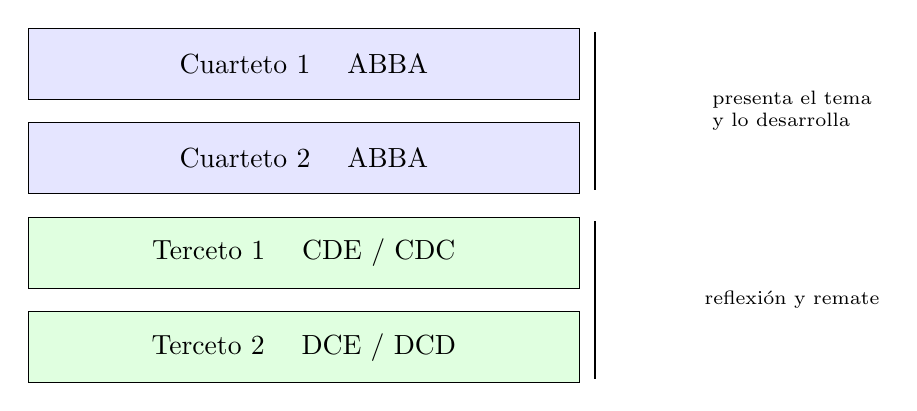
\begin{tikzpicture}
\tikzset{every node/.append style={align=center}}

\node[draw, fill=blue!10, minimum width=7cm, minimum height=0.9cm] (c1) at (0,3.6) {Cuarteto 1 \quad ABBA};
\node[draw, fill=blue!10, minimum width=7cm, minimum height=0.9cm] (c2) at (0,2.4) {Cuarteto 2 \quad ABBA};
\node[draw, fill=green!12, minimum width=7cm, minimum height=0.9cm] (t1) at (0,1.2) {Terceto 1 \quad CDE / CDC};
\node[draw, fill=green!12, minimum width=7cm, minimum height=0.9cm] (t2) at (0,0) {Terceto 2 \quad DCE / DCD};
\node[align=left, font=\scriptsize] at (6.2,3.0) {presenta el tema\\ y lo desarrolla};
\node[align=left, font=\scriptsize] at (6.2,0.6) {reflexión y remate};
\draw[thick] (3.7,2.0) -- (3.7,4.0);
\draw[thick] (3.7,-0.4) -- (3.7,1.6);

\end{tikzpicture}
\end{document}
